\documentclass[12]{article}

\usepackage{geometry}
\usepackage{amsmath, amsthm, amssymb}
\usepackage{graphicx}
\usepackage{tikz}
\usepackage{booktabs} % See the package documentation for guidelines on formal tables: https://ctan.org/pkg/booktabs
\usepackage{verbatim} % Used to typeset, for example, code snippets or pseudo-code for algorithms.
\usepackage{dsfont} % Extra fontset for helpful mathematics symbols, e.g. \mathds{1}
\usepackage{etoolbox} % Used to allow boolean variables for use in the title page
\usepackage{import}
\usepackage{lipsum}
\usepackage{subcaption}
\usepackage{float}
\usepackage{enumitem}
\usepackage{tabularx}
\usepackage{array}
\usepackage{pdfpages}
\usepackage{mathtools}
\usepackage{hyperref}
\usepackage{bbm}
\newcolumntype{C}[1]{>{\centering\arraybackslash}m{#1}}

%\setlength{\parskip}{\baselineskip}%
%\setlength{\parindent}{0pt}%

\newcommand{\R}{\mathbb{R}}
\newcommand{\Q}{\mathbb{Q}}
\newcommand{\C}{\mathbb{C}}
\newcommand{\N}{\mathbb{N}}
\newcommand{\Z}{\mathbb{Z}}
\newcommand{\T}{\mathbb{T}}
\newcommand{\cA}{\mathcal{A}}
\newcommand{\cB}{\mathcal{B}}
\newcommand{\cD}{\mathcal{D}}
\newcommand{\cP}{\mathcal{P}}
\newcommand{\cM}{\mathcal{M}}
\newcommand{\abs}[1]{\left\lvert #1 \right\rvert}
\newcommand{\norm}[1]{\left\lVert #1 \right\rVert}
\newcommand{\set}[2]{\left\{#1 \ : \ #2\right\}}
\newcommand{\conv}[1]{\underset{#1}\longrightarrow}
\newcommand{\Mod}[1]{\ (\mathrm{mod}\ #1)}
\newcommand{\Supp}[0]{\ \mathrm{Supp}\ }
\DeclarePairedDelimiter\ceil{\lceil}{\rceil}
\DeclarePairedDelimiter\floor{\lfloor}{\rfloor}
\DeclareMathOperator{\lcm}{lcm}
\newcommand{\Cross}{\mathbin{\tikz [x=1.4ex,y=1.4ex,line width=.2ex] \draw (0,0) -- (1,1) (0,1) -- (1,0);}}

\newcommand\restr[2]{{% we make the whole thing an ordinary symbol
		\left.\kern-\nulldelimiterspace % automatically resize the bar with \right
		#1 % the function
		\vphantom{\big|} % pretend it's a little taller at normal size
		\right|_{#2} % this is the delimiter
}}
% Custom math operators (analogous to \lim, \sup, etc).
\DeclareMathOperator{\id}{id}
\DeclareMathOperator{\subspan}{span}
\DeclareMathOperator{\sgn}{sgn}
\DeclareMathOperator{\diam}{Diam}
\DeclareMathOperator{\mult}{mult}

\newtheorem{thm}{Theorem}[section] % Numbering is impacted by [chapter]; could do [section] or [subsection] also.
\newtheorem{lem}{Lemma} % The [thm] argument says to number Lemma in sequence with Theorem.
\newtheorem{prop}[thm]{Proposition}
\newtheorem{cor}[thm]{Corollary}
\newtheorem{conj}[thm]{Conjecture}
\newtheorem{question}{Question}
% These environments are unnumbered and will not count toward the numbering.
%\newtheorem*{question}{Question}
\newtheorem*{answer}{Answer}
\newtheorem*{conjecture}{Conjecture}
\newtheorem*{claim}{Claim}
% These environments are definitions; they have a different style (bold label, standard font).
\theoremstyle{definition}
\newtheorem{defn}[thm]{Definition} % These definitions are also numbered in sequence with Theorem.
\newtheorem{eg}{Example}
\newtheorem{rem}[thm]{Remark}
\newtheorem{obs}{Observation}

\title{ \vspace{-3cm} CanaDAM 2023 }
\author{Tao Gaede}

\begin{document}
	\maketitle
	\tableofcontents
	
	\newpage
	\section{Monday:}
	\subsection{Morning}
	
	\paragraph{8:30 IS (MET):} Hypergraphs, topology and resource allocation.
	Matchings in hypergraphs using topological methods.
	
	-
	
	-
	
	\paragraph{10:00 CM24 (1L04):} Second largest eigenvalue of trees.
	Extremal trees of order n and diameter d that maximize second largest eigenvalue.  Probably relevant my work on distances in trees.
	
	-
	
	-
	
	\paragraph{10:30 IM2:} Intersecting families of sets are typically trivial.
	Improved bound $k > k_0$ for k-intersecting families whereby the families tend to be stars (trivial).  Interesting to get background on intersecting families.  While stars may be common, what types of intersecting families are uncommon?  Is there a common uncommon intersecting family, or do we not know much about the uncommon ones?  Maybe get a better sense for what other structure is needed to make them applicable to tone networks.
	
	-
	
	-
	
	\paragraph{*11:00 CM24:} Packings of Partial Difference Sets.
	Might be over my head, but I'm curious about difference sets.
	
	-
	
	-
	
	\paragraph{*11:00 CT:} The exact threshold for zero sum cycles in complete diagraphs.
	They find the exact smallest number n such that for every Zq - arc labelling of a complete digraph of order n, there is a directed cycle whose arc labels sum to 0.  I feel like this could have relevence to handling distance summation issues that arrise in edge-labelled graphs.
	
	\paragraph{11:30 IM2:} The Burning Number Conjecture holds asymptotically.
	The burning number refers to smallest k such that a graph G of order n can be covered by balls of radii 0, 1, ..., k.  This interval of radii condition is slightly similar to the interval multiplicity condition in crescent configurations.  Perhaps there's overlap.
	
	-
	
	-
	
	\begin{center} 
		\item\paragraph{\underline{Things to look into}} 
	\end{center}

	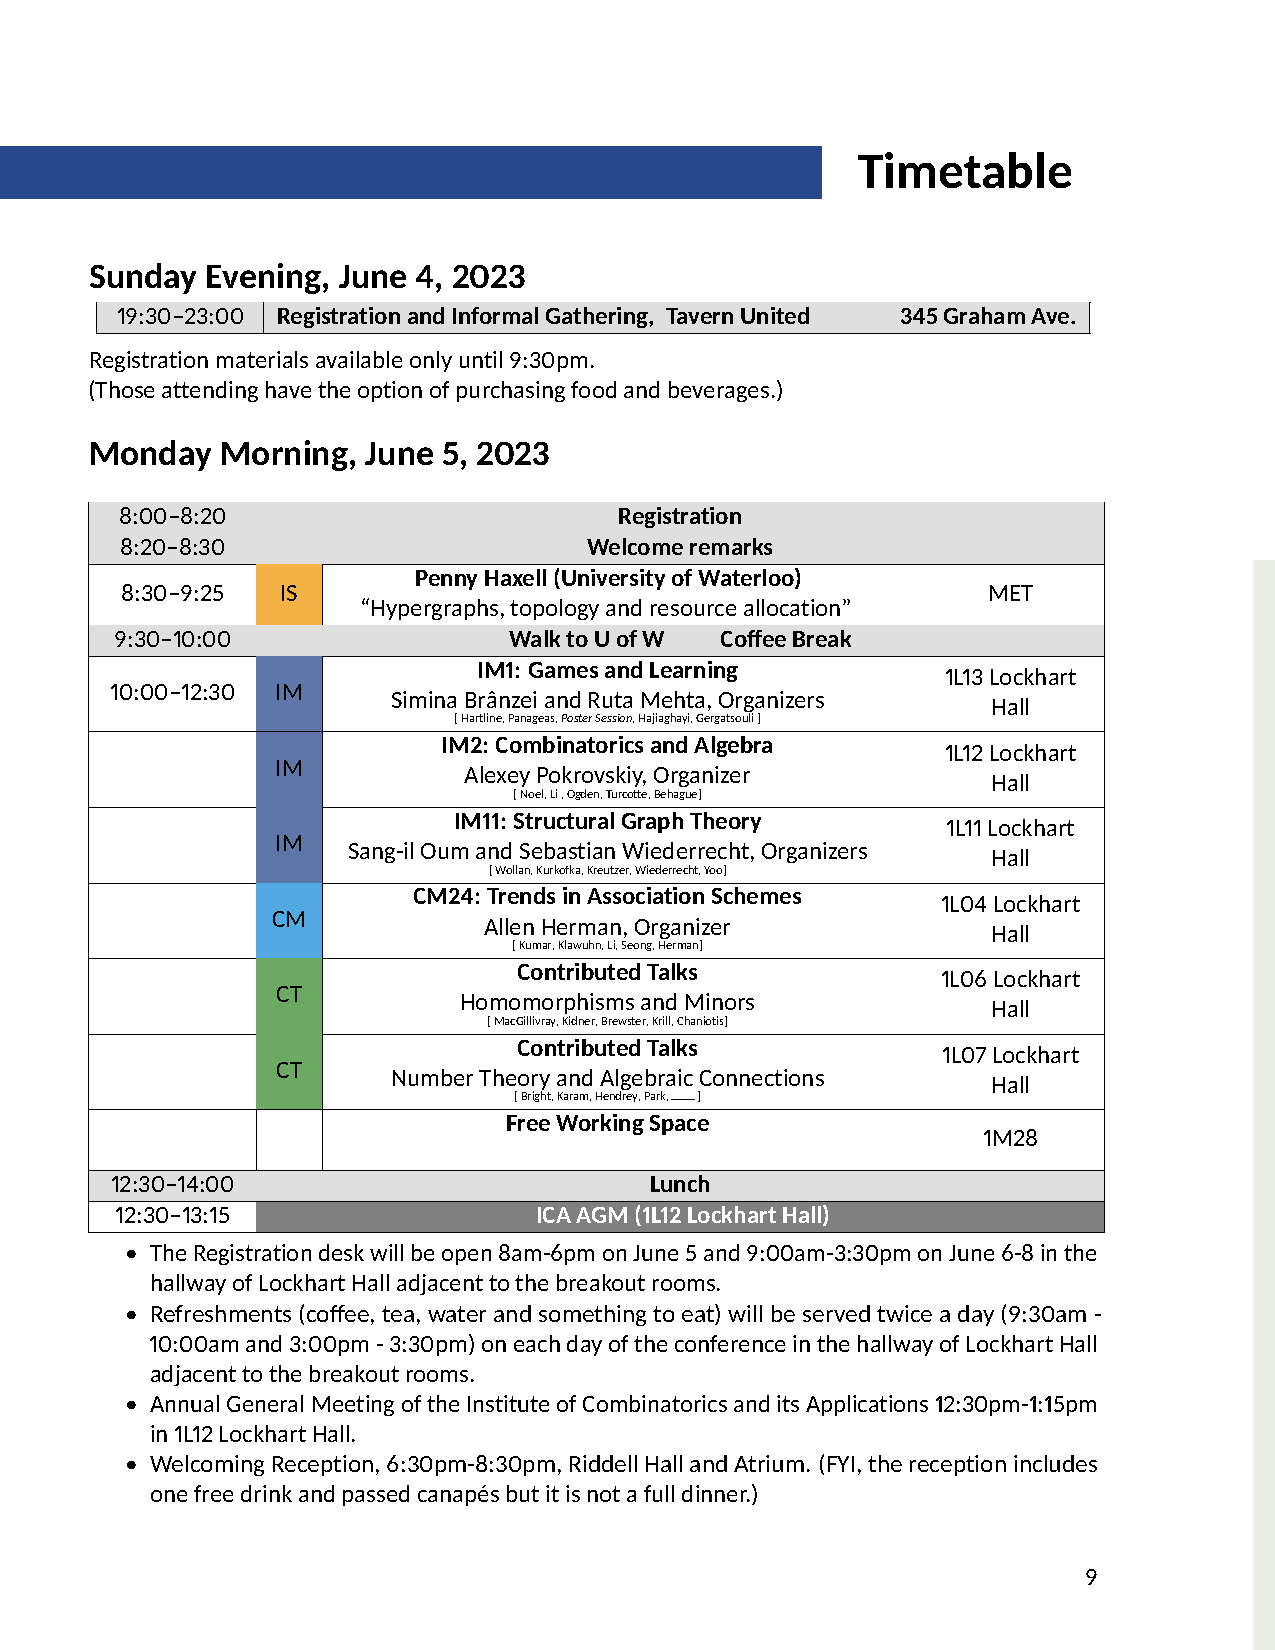
\includepdf[pages=1]{CanaDAM-program.pdf}
	\newpage
	\subsection{Afternoon}
	
	\paragraph{2:00 IS (MET):} A random Hall-Paige Conjecture.
	About transversals in group multiplication tables.  Uses probabilistic methods.
	
	-
	
	-
	
	\paragraph{3:30 CM13 (1L11):} Turan and Ramsey-type problems for affine structures.
	I haven't seen a lot of this before, but it involves some extremal questions on finite fields, which seems interesting.
	
	-
	
	-
	
	\paragraph{4:00 CM21 (1L08):} The one-visibility localization game.
	To get my feet wet in some cops and robbers.  The robber is invisible, and a set of cops try to find the location of the robber.
	
	-
	
	-
	
	\paragraph{4:30 CM20 (1L07):} A balancing act on matrices.
	Integer matrices and decompositions.  I'm curious about graph decomposition problems and I'm interested to learn more about properties of integer matrices.
	
	-
	
	-
	
	\paragraph{5:00 CT (1L06):} Graph-theoretical questions arising from DNA self-assembly.
	Presents combinatorial representations of DNA structures, which could give me a better sense for how to link my interest in biochemistry with combinatorics and graph theory.
	
	-
	
	-
	
	\paragraph{5:30 CM13 (1L11):} Unit and distinct distances in typical norms.
	Directly related to Erdos distinct distances problem in the plane.
	
	-
	
	-
	
	\begin{center} 
		\item\paragraph{\underline{Things to look into}} 
		\end{center}
	
	\includepdf[pages=2]{CanaDAM-program.pdf}
	\newpage
	\section{Tuesday:}
	\subsection{Morning}
	\paragraph{8:30 IS (MET):} Sampling and high-dimensional expansion
	
	-
	
	-
	
	\paragraph{*10:00 CT (1L06):} Time delayed Cops and Robber.
	
	-
	
	-
	
	\paragraph{*10:00 CM22 (1L04):} Perfect state transfer on trees with small diameter.
	Maybe I'll learn something about quantum information theory.
	
	\paragraph{*10:30 CM22 (1L04):} Classes of trees without perfect state transfer.
	More QIT.
	
	-
	
	-
	
	\paragraph{*10:30 IM9 (1L12):} Combinatorial characterization of the exact rank of sparse random matrices.  What is the rank of the adjacency matrix of G(n,p)?
	
	\paragraph{*10:30 CT (1L06):} Perfect 1-factorisations of hypergraphs.
	
	\paragraph{11:00 CT (1L06):} Large k-sparse sets in triangle-free graphs.
	
	-
	
	-
	
	\paragraph{11:30 CT (1L06):} On the decomposability of codes with embedded (6L-2, 2L, L)-designs.
	
	-
	
	-
	
	\paragraph{12:00 (1L06):} Subdivision and adjacency spectra of graphs.
	Subdividing a subset of edges of a graph, and proving things about the eigenvalues of the adjacency matrix for the resulting graph.  The sequence St of the k-th eval for the graph with subdivision lengths t, is shown to be Cauchy.  It could be interesting to see some analysis relating to graphs.
	
	-
	
	-
	
	\begin{center} 
		\item\paragraph{\underline{Things to look into}} 
	\end{center}

	\includepdf[pages=3]{CanaDAM-program.pdf}
	\newpage
	\subsection{Afternoon}
	
	\paragraph{2:00 IS (MET):} On the simplex method and diameter of 0/1 polytopes
	
	-
	
	-
	
	\paragraph{*3:30 IM10 (1L12):} Complexes of nearly maximum diameter.
	
	-
	
	-
	
	\paragraph{*3:30 CM21 (1L08):} Firefighting with a distance-based restriction.
	
	\paragraph{*4:00 (1L06):} Distance-preserving graph compression techniques.
	Might provide insight on how to add/remove edges of trees while minimizing changes in distance multiplicities.
	
	-
	
	-
	
	\paragraph{*4:00 CM21 (1L08):} A two player graph burning game.
	
	\paragraph{4:30 CM21 (1L08):} Extending graph burning to hypergraphs.
	
	-
	
	-
	
	\paragraph{5:00 CM21 (1L08):} Herding cats stuck in trees.
	
	-
	
	-
	
	\paragraph{5:30 CM21 (1L08):} The watchman's walk problem on Cayley graphs.
	
	-
	
	-
	
	\begin{center} 
		\item\paragraph{\underline{Things to look into}} 
	\end{center}

	\includepdf[pages=4]{CanaDAM-program.pdf}
	\newpage
	\section{Wednesday:}
	\subsection{Morning}
	
	\paragraph{8:30 IS (MET):} The sharp power law of local search on expanders.
	
	-
	
	-
	
	\paragraph{10:00 CM16 (1L11):} Separating the edges of a graph by a linear number of paths.
	
	-
	
	-
	
	\paragraph{10:30 CM16 (1L11):} Improved bounds for cross-Sperner systems.
	
	-
	
	-
	
	\paragraph{11:00 IM9 (1L12):} A simple and sharper proof of the hypergraph Moore bound.
	
	-
	
	-
	
	\paragraph{*11:30 IM6 (1L08):} The existence of subspace designs.
	
	-
	
	-
	
	\paragraph{*11:30 CM16 (1L11):} Invertibility of digraphs and tournaments.
	
	\paragraph{12:00 CT (1L06):} Rainbow 3-partite graphs.
	
	-
	
	-
	
	\begin{center} 
		\item\paragraph{\underline{Things to look into}} 
	\end{center}

	\includepdf[pages=5]{CanaDAM-program.pdf}
	\newpage
	\subsection{Afternoon}
	
	\paragraph{2:00 IS (MET):} Quadratic forms and clique-free graphs.
	
	-
	
	-
	
	\paragraph{*3:30 IM3 (1L07):} New results on skew and strong frame starters in cyclic groups.
	
	-
	
	-
	
	\paragraph{*3:30 IM8 (1L08):} A colorful Borsuk-Ulam theorem.
	
	\paragraph{*3:30 CT (1L06):} Using alternating de Bruijn sequences to generate de Bruijn tori.
	
	\paragraph{4:00 CT (1L06):} Avoiding additive powers in words.
	
	-
	
	-
	
	\paragraph{4:30 CT (1L06):} Structural characterization of connected graphs with integer-valued Q-spectral radius.
	
	-
	
	-
	
	\paragraph{5:00 IM3 (1L07):} Value distributions of perfect nonlinear functions.
	
	-
	
	-
	
	\paragraph{5:30 IM8 (1L08):} Rigidity expander graphs.
	
	-
	
	-
	
	\begin{center} 
		\item\paragraph{\underline{Things to look into}}
	\end{center}

	\includepdf[pages=6]{CanaDAM-program.pdf}
	
	\newpage
	\section{Thursday}
	
	\subsection{Morning}
	
	\paragraph{8:30 IS (MET):} Catalanimals.
	
	-
	
	-
	
	\paragraph{10:00: CM19 (1L12):} The threshold strong dimension of a graph.
	
	-
	
	-
	
	\paragraph{*10:30 CM14 (1L08):} Approximative cycle double cover.
	
	-
	
	-
	
	\paragraph{*10:30 CM19 (1L12):} On the threshold strong dimension of the n-cube.
	
	\paragraph{11:00 CM19 (1L12):} Metric dimension parameterized by feedback vertex set and other structural parameters.
	
	-
	
	-
	
	\paragraph{11:30 CM19 (1L08):} Metric dimension of growing infinite graphs.
	
	-
	
	-
	
	\paragraph{*12:00 CM16 (1L11):} Enumerating graphic sequences.
	
	-
	
	-
	
	\paragraph{*12:00 CM14 (1L08):} Some new results on vertices belonging to all metric bases.
	
	\begin{center} 
		\item\paragraph{\underline{Things to look into}} 
	\end{center}

	\includepdf[pages=7]{CanaDAM-program.pdf}
	\newpage
	
	\subsection{Afternoon}
	\paragraph{2:00 IS (MET):} Poset inequalities
	
	-
	
	-
	
	\paragraph{3:30 IM3 (1L07):} Small difference sums for dense packings.
	
	-
	
	-
	
	\paragraph{4:00 IM3 (1L07):} Generalisations of bipartite graph designs.
	
	-
	
	-
	
	\paragraph{*4:30 IM3 (1L07):} Intersecting sets of uniform partitions.
	
	-
	
	-
	
	\paragraph{*4:30 CM23 (1L13):} Monochromatic sums and products over the rationals.
	
	\paragraph{*5:00 IM3 (1L07):} Extending difference matrices over abelian p-groups.
	
	-
	
	-
	
	\paragraph{*5:00 IM8 (1L08):} A positive answer to Barany's question on face numbers of polytopes.
	
	\paragraph{*5:30 IM3 (1L07):} Cover-free families on hypergraphs.
	
	-
	
	-
	
	\paragraph{*5:30 CM23 (1L13):} Off-diagonal poset Ramsey numbers.
	
	\begin{center} 
		\item\paragraph{\underline{Things to look into}} 
	\end{center}

	\includepdf[pages=8]{CanaDAM-program.pdf}

\end{document}
